\chapter{外文资料的调研阅读报告或书面翻译}
\label{cha:CN}
\title{Zooids: 用于集群交互的积木}

\begin{figure}[htbp]
    \centering
    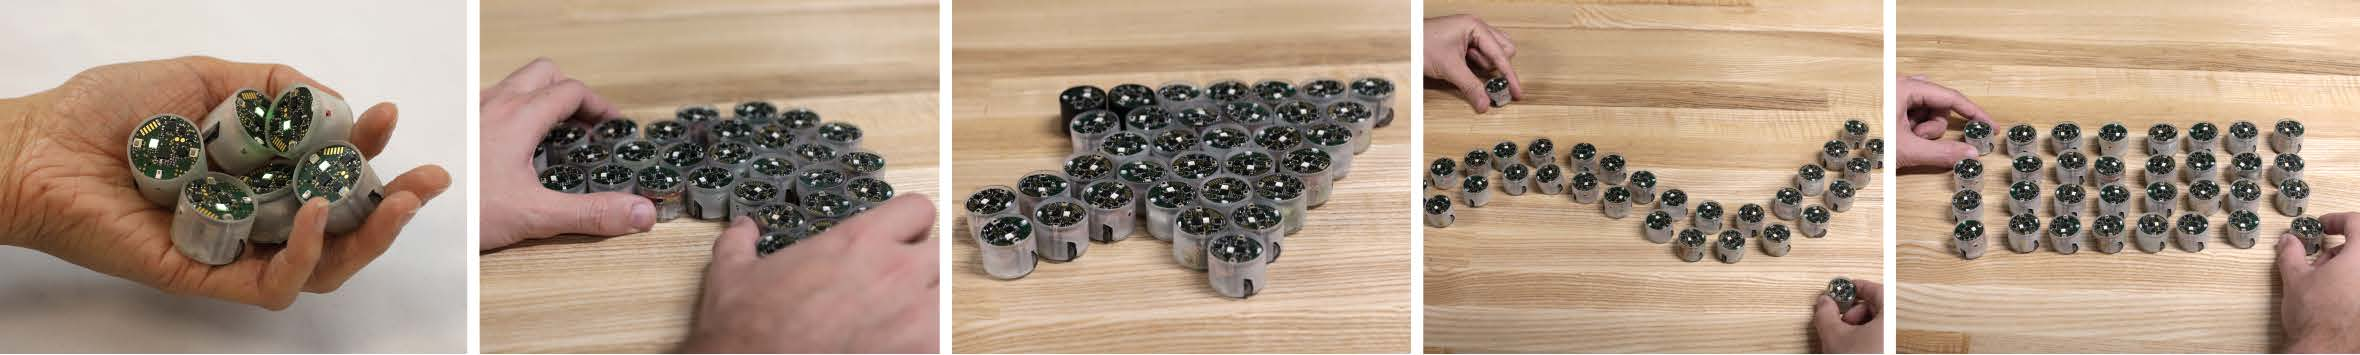
\includegraphics{zooids-1.jpg}
    \caption*{图~1\hskip1em Zooids可以被持有,可以集体或单独被操纵,表现为物理像素,充当控制器,并且可以在控制下动态移动。 它们是被称为群体交互界面的新型用户界面的积木单元。}
    \label{fig:headfigure}
\end{figure}

{\heiti 摘要:} 本文介绍了集群交互,这是一类新型的人机界面,由许多能够显示和交互的自主机器人组成。我们设计的Zooids是用于开发桌面集群交互的开源软硬件平台。该平台包括一组直径为2.6 cm的定制设计轮式微型机器人,一个无线电基站,一个用于光学跟踪的高速DLP结构光投影仪以及一个用于应用程序开发和控制的软件框架。我们通过使用Zooids开发的一组应用场景说明了桌面集群交互用户界面的潜力,并讨论了集群交互用户界面特有的设计注意事项。

{\heiti 关键词:} 集群用户界面; 实物用户界面。

\section{简介}

